\chapter{Projectile Motion and Conservation of Energy}
\label{chap:projectile}
\section{Introduction}
In this experiment, we use the trajectory equations of a body in two-dimensional free fall to predict where a projectile hits the ground\footnote{See Sections 4-5, 4-6 of \emph{Fundamentals of Physics} by Halliday, Resnick \& Walker.}. The initial (launch) velocity of the projectile is determined by applying the law of conservation of energy\footnote{Chapter 8 of Halliday, Resnick \& Walker.} for the projectile traveling through a long bent tube. We compare the predicted and measured location after the fall. This lab should demonstrate the predictive power of applying physical principles correctly, show that predictions correspond to something in the ``real world'', and provide insight about deciding what is important in making a measurement.\myskip

\underline{\emph{Remark}:} You must prepare some derivations at home; otherwise, you may have trouble finishing the lab in the time given.

\section{Theory}
\subsection{Conservation of Energy}
One of the most fundamental principles of physics requires that total energy be conserved in all physical processes. This principle is sometimes difficult to apply since there are many different kinds of energy (potential energy, kinetic energy, rotational energy, heat, chemical energy, and mass\footnote{This is the content of Einstein's famous formula: $E=mc^2$!}), and energy can be transformed from one kind to another. We will deal primarily with the first three types of energy, and with a small loss due to friction (which usually ends up converted into heat). In the previous lab you saw how conservation of momentum is sometimes more useful than conservation of energy; in this lab, we will focus on a situation where conservation of energy is the appropriate law to use.\myskip

The kinetic energy of a point particle moving with velocity $v$, is given by $E_{\textrm{Kin}}=mv^2/2$. Because the rolling ball used in this experiment is not a point object, we need to take into account its rotational motion. This is discussed in the next section. \myskip

The potential energy for an object near the earth’s surface is given by $E_{\textrm{Pot}}=mgh$, where $h$ is the height above an arbitrarily chosen level. This means that when an object drops from a vertical height $h_2$ to $h_1$, $\Delta h=h_1-h_2$, the loss in potential energy is $mg\Delta h$.\myskip

Some energy is always lost due to friction. If we label the friction energy loss $W$, it follows that:
\begin{equation}
\textrm{\emph{Gain in K.E.}} = (\textrm{\emph{P. E. lost}}) - W
\end{equation}

\subsection{Estimating the Friction Loss}

If there were no friction, all the loss in potential energy ($mg\Delta h$), as the ball rolls from the release point to the launch point, would be converted to kinetic energy. However, because of friction, some of the energy will be dissipated. We need a technique to determine the energy lost to friction. Here, we find the orientation of the track such that that when released from the top, the ball just comes to rest at the lower end of the track. When the ball comes to rest, we know that the kinetic energy is zero, so the difference in potential energy between the initial and final positions must have all been lost to friction. Then, we determine the vertical distance traveled by the ball $\Delta h'$ and $mg\Delta h'$ equals the energy lost to friction. If we assume that the same amount of energy is lost to friction when the track is tilted more steeply, we can use $W=mg\Delta h'$ for all tilts. It follows that:
\begin{align}
  \textrm{\emph{Gain in K.E.}}&=(\textrm{\emph{F.E. lost}})-W\\
  &=mg\Delta h-mg\Delta h'\\
  &=mg(\Delta h-\Delta h')
\end{align}

\underline{\emph{Remark}:} There are three types of ball in the experiment: steel (or brass), aluminum and plastic. You have to measure the friction separately for each ball!

\subsection{Kinetic Energy including Rotation}

In this experiment, we deal with a rolling ball. We need to account for the rolling motion, so that there are two contributions to the kinetic energy:
\begin{equation}
  \textrm{\emph{Kinetic Energy}} = \textrm{\emph{Kinetic Energy of center of mass}}+\textrm{\emph{Kinetic Energy of rotation}}
\end{equation}

This relationship takes the analytic form:
\begin{equation}
  E_{\textrm{Kin}}=\frac{1}{2}mv^2+\frac{1}{2}I\omega^2
\end{equation}
where $m$ is the total mass of the object, $v$ is the velocity of the center of mass, $I$ is the moment of inertia ($I = 2m R^2/5$ for a sphere), and $\omega$ is the angular velocity of rotation. (For a rolling ball that is not sliding, $\omega=v/R$). The total kinetic energy of the rolling sphere is:
\begin{align}
  E_{\textrm{Kin}}&=\frac{1}{2}mv^2+\frac{1}{2}\bigg(\frac{2}{5}mR^2\bigg)\bigg(\frac{v}{R}\bigg)^2\\
  E_{\textrm{Kin}}&=\frac{1}{2}mv^2+\frac{1}{5}mv^2\\
  E_{\textrm{Kin}}&=\frac{7}{10}mv^2
\end{align}

As can be seen from the final result, the kinetic energy of a rolling ball is slightly larger than that of a point object travelling at the same speed\footnote{If you have not yet had rotations in lecture, you may not follow this argument in detail. But the last equation indeed does express the kinetic energy of the rolling ball (see HRW Section 11-3). Be sure to use it.}.

\subsection{Parabolic Trajectory}
The motion of a mass launched into free fall with initial velocity, $v$, at an angle $\varphi$ relative to the horizontal, can be treated most easily by evaluating the horizontal (or $x$) and vertical (or $y$) position in terms of the time ($t$) as two independent motions. This problem, in which explicit expressions for $y(t)$ and $x(t)$ are obtained has been treated in your text and in lecture. (We neglect air resistance while the ball is in free fall.)

\section{Procedure}
Figure \ref{fig:apparatus} shows the apparatus to be used in this experiment. A ball is released into a tube at the release point, rolls through the tube and emerges at the launch point. You need to measure all parameters shown explicitly in the figure ($h_1, h_2, h_3, D, L$), and the additional parameter, $\Delta h'$, which is used to estimate friction losses.\myskip

\underline{\emph{Remark}:} If you want to clean the tube beforehand (which will reduce error in the experiment), there should be a swab on a string available.\myskip
\begin{figure}[h]
\centering
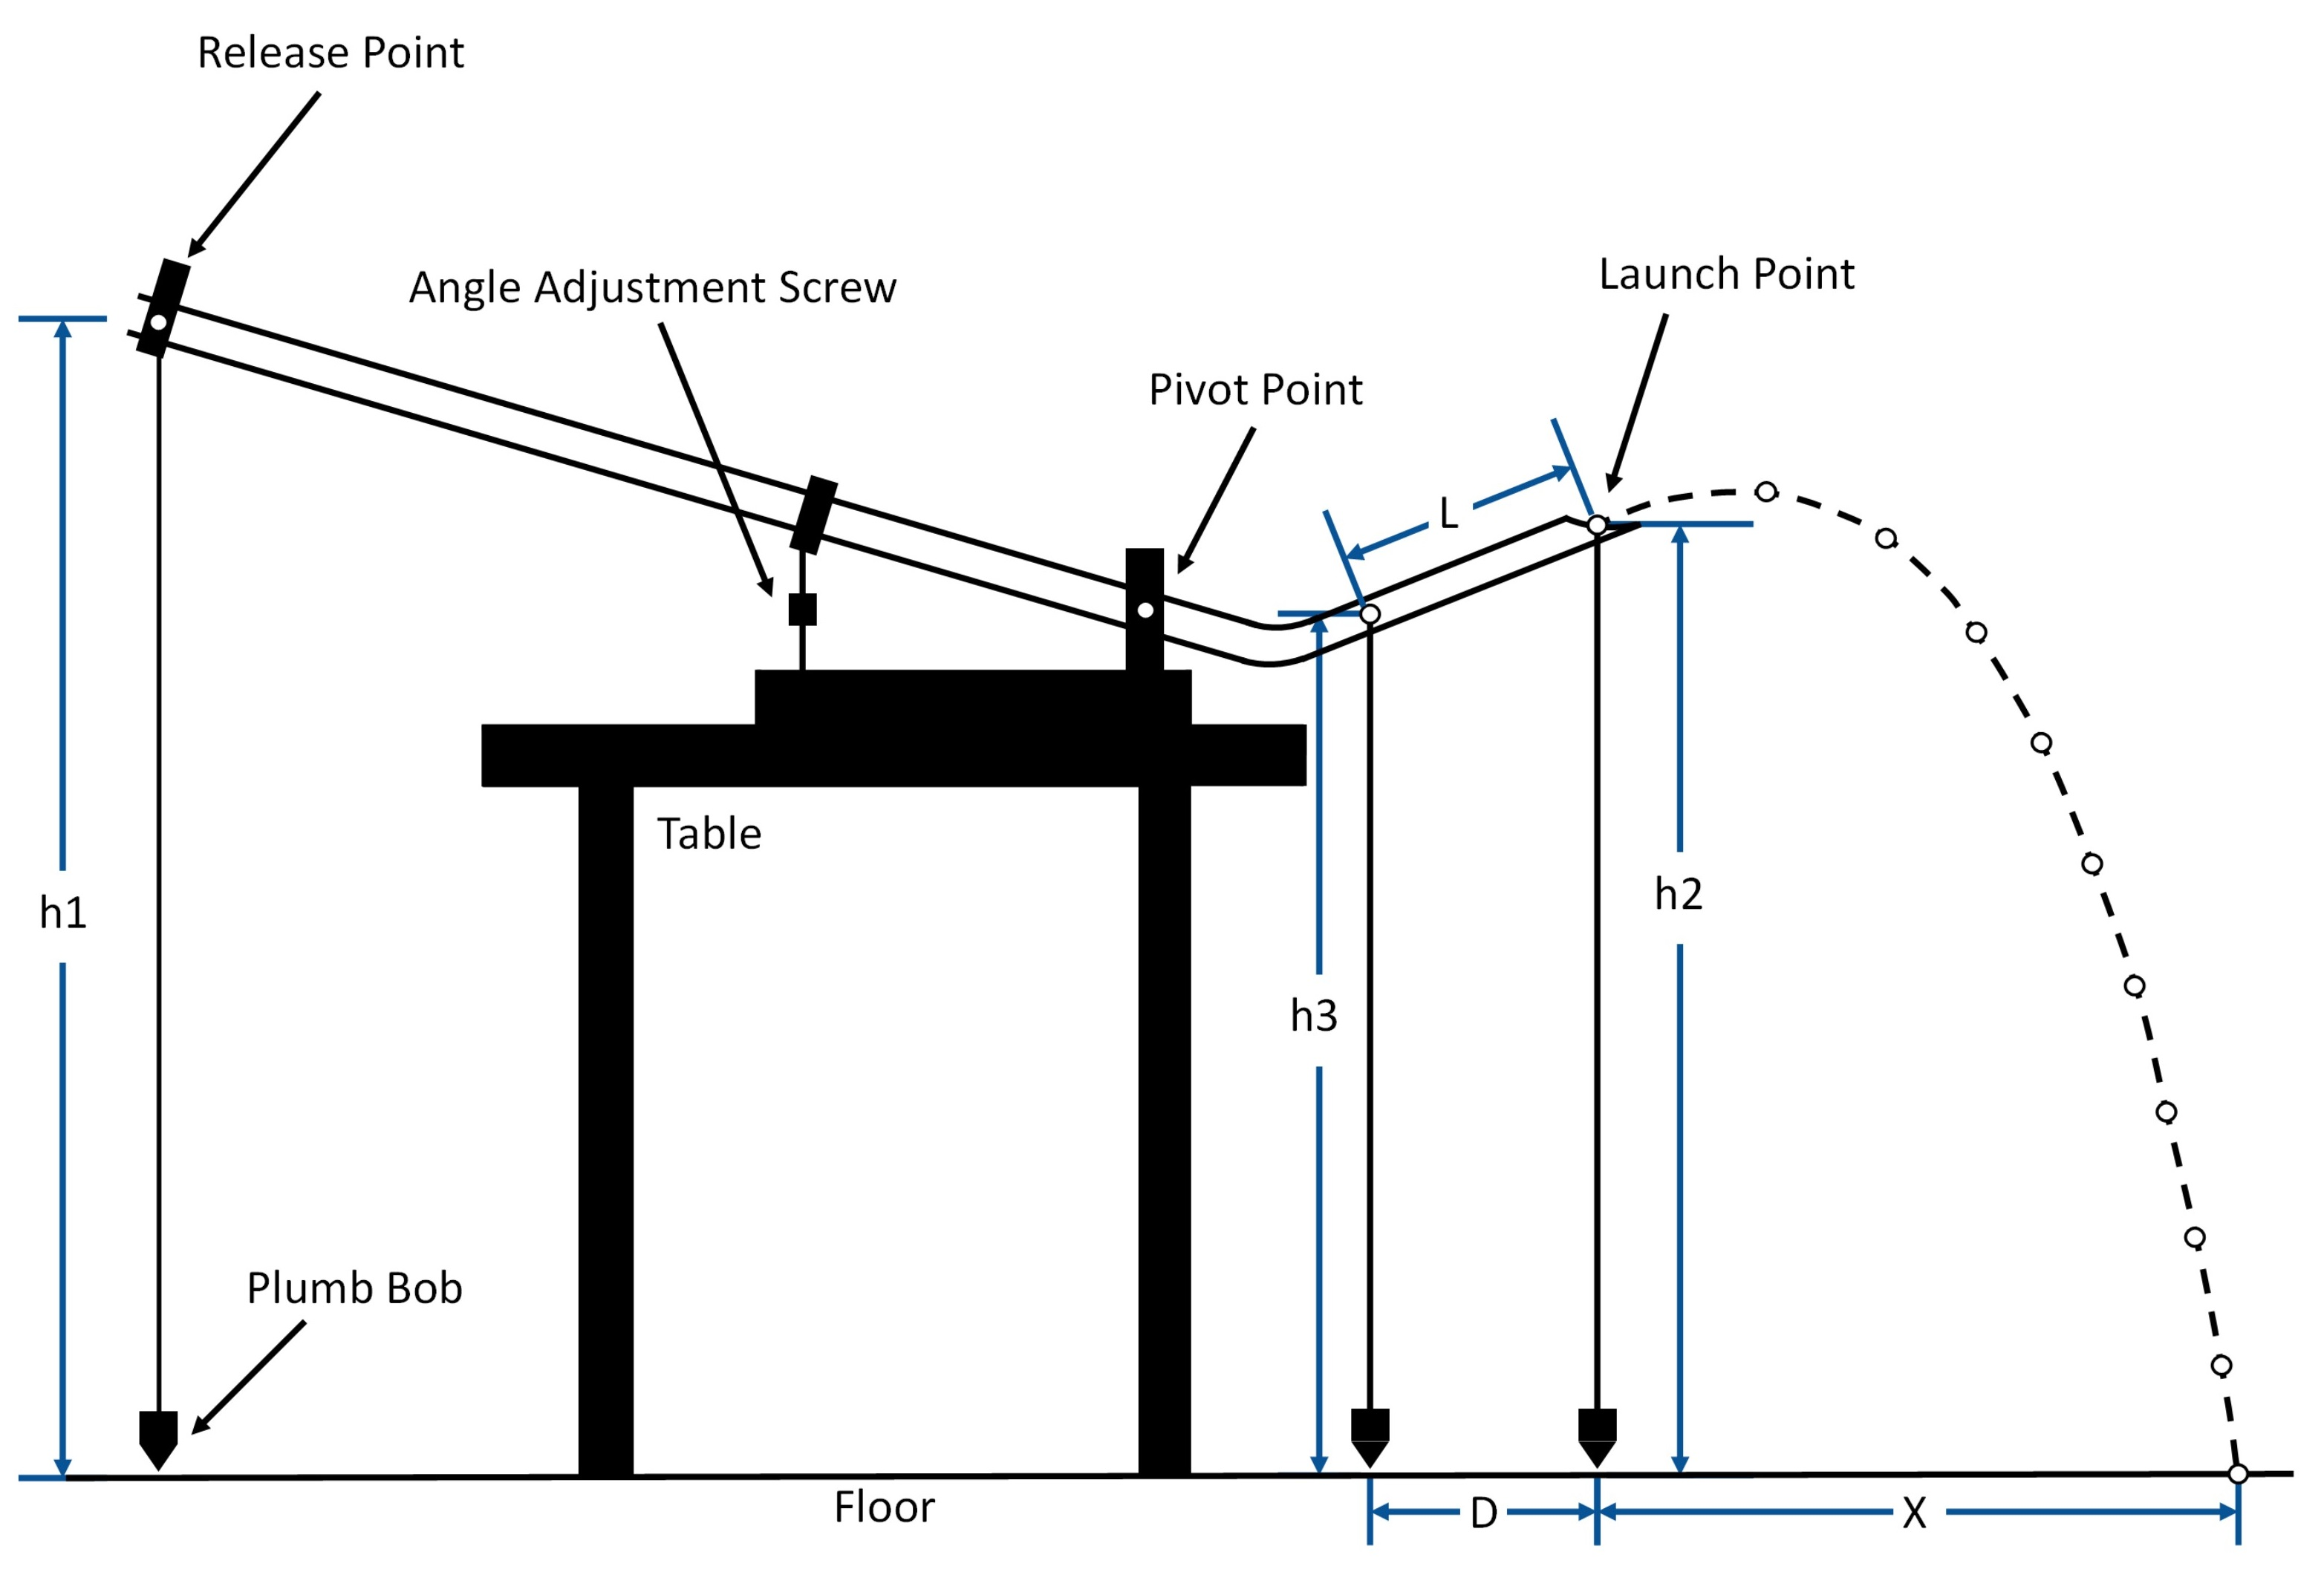
\includegraphics[width=1.0\textwidth]{./Exp4/pic/image11.jpg}
\caption{The Apparatus}
\label{fig:apparatus}
\end{figure}

\subsection{Prediction of Position}
Before you do the experiment, you should derive a set of equations at home that predict the $x$-position where the ball hits the ground ($y=0$). This expression should depend only on the measured parameters shown in the figure: $h_1$, $h_2$, $h_3$, $D$, $L$, as well as the value of $\Delta h'$. You will need to substitute these quantities rather than parameters we do not directly measure, like $v$, $\sin(\theta)$, or $\cos(\theta)$.\myskip

Rather than derive a single complicated formula for the range of the projectile $x$ in terms of symbols for all the preliminary measurements, it is more convenient to calculate, in sequence, several intermediate quantities and then combine them to find the range $x$. Bring the sheet with your derivation of the formulae for $x$ in terms of the measured parameters. You should prepare this before coming to the lab!  It should be attached to the report when you are finished.
\begin{enumerate}
\item Find  the magnitude of the launching velocity $v$ by using the conservation of total mechanical energy (incorporating the estimate of the energy lost to friction).
\item Find the horizontal velocity $v_x$ and vertical velocity $v_y$ by referring to the geometry of the final section of the track.
\item Find the time the ball is in the air $t$ by considering the vertical motion involving $v_y$ and $h_2$ alone.
\item Finally, find the range $x$.
\end{enumerate}

Steps 3 and 4 may be combined by using the trajectory equation $y(x)$, obtained by eliminating the time in the equations for $y(t)$ and $x(t)$.\myskip

\subsection{Verify your Range Expression}
Now, you will verify the validity of your range expression by looking at the trajectories of two spheres (we suggest using the heavy metal ball and the plastic balls). Start with the plastic ball.
\begin{enumerate}
\item Adjust the angle adjustment screw such that the ball, when released at the release point, {\it{just makes it to the launch point}} before reversing direction. This gives us an estimation of the enegy lost due to friction.
\item Record $h_1'$, $h_2'$, and $\Delta h'$.
\item Increase $h_1$ with the adjustment screw so that the ball will be launched. Make sure that that $h_1-h_2$ is at least twice as big as $h_1'-h_2'$.
\item Measure all the required quantities and predict where the ball will hit the floor. Place a coin at that position. Release the ball and see if the ball hits the coin.

\item Repeat setps 1-4 for the heavy metal ball with the same launching $h_1$, $h_2$, and $h_3$ (re-measure all relevant quantities).
\item Did the spheres land where you expected? If not, what errors may have caused the discrepancy?
\item The difference $\Delta h'’= h_1' - h_2'$ provides a comparitive measure of the energy lost to friction as the ball traverses the tube. Order the measurements of the spheres from highest to lowest $\Delta h'$. Explain why you might have expected this order.
\item Which ball would you have expected to fly the furthest horizontal distance from the same release point? Why?
\item Quantitatively discuss how far off would your results be if you had not corrected for the friction losses in the tube (recalculate the range $x$ for both spheres setting $\Delta h'=0$)?
\item From the comparison of your results with the predictions, do you think ignoring air resistance contributed to the error? How do you expect air resistance to affect the range?
\end{enumerate}

\subsection{Quantitative Measurements and Uncertainty}
In this part of the experiment, you will take measurements of the hit position relative to that predicted. These data will permit a measure of the spread, or uncertainty, from the reproducibility of the results. You will take measurements for two balls (heavy metal and plastic) for the same orientation of the launching tube.\myskip

Place a sheet of white paper on the floor centered at the predicted location and place a piece of carbon paper on top of it (make sure to tape both pieces of paper to the floor). Before proceeding, make a guess of how large the spread of results will be!\myskip

Roll a single ball about twenty times using the heights ($h_1$, $h_2$, and $h_3$); you should obtain the same number of points marked on the white paper. These should be spread around the expected value. Do this experiment with different papers for the heavy metal ball and for the plastic ball.
\begin{enumerate}
    \item How do you expect the spread of measurements to appear? (Qualitatively, not quantitatively!)
    \item Describe and compare the two spreads. (How large is the spread?  Is it uniform in all directions? Should it be?  Is the spread the same for both balls? Should it be? Is the spread about as big as you expected?)
    \item If the spread is much bigger along the direction of the trajectory than perpendicular to it, how would you interpret this?
    \item Make a few suggestions for how you could have improved the first part of the experiment so that you would always hit a smaller area, like that of a dime!
\end{enumerate}

\subsection{Checking Formula}
If you want to check if your derived formula for the position where the projectile hits the ground is correct, you can use the following data:
\begin{table}[h]
  \centering
  \begin{tabular}[h]{r@{=}r@{.}lcr@{=}r@{.}l}
    $h_{1}$&124&3 cm&&$h_{3}$&110&0 cm\\
    $h_{1}'$&122&7 cm&&D&27&7 cm\\
    $h_{2}$&119&3 cm&&L&29&2 cm\\
    $h_{2}'$&120&5 cm
  \end{tabular}
\end{table}
The position the projectile hits the ground is then at: $x  =  30.5\, \textrm{cm}$.

\section{Lab Preparation Examples}

\myskip
{\bf{Note: Suggested prelab questions are in bold. These will help will conceptual understanding of the laboratory experiments. }}
\myskip

\noindent\underline{Trajectories}:
\myskip
{\bf{1. What is your predicted value for $x$, assuming you measure the following values:}}
\begin{table}[h]
  \centering
  \begin{tabular}[h]{c@{=}ccc@{=}ccc@{=}c}
    $h_{1}'$&105 cm&&$h_{2}'$&90 cm&\\
    $h_{1}$&120 cm&&$h_{2}$&80 cm&&$h_{3}$&65 cm\\
    L&25 cm&&$D$&20 cm&
  \end{tabular}
\end{table}

2. If $h_1' = 125\, \textrm{cm}$ and $h_2'  = 100\, \textrm{cm}$, what percentage of the potential energy is lost to friction?\myskip

{\bf{3. You shoot a bullet with velocity $v$ and an angle $\varphi$ to the horizontal direction and observe where it hits the ground. You now increase the angle with which a bullet is shot. Does it reach further or not?  Does the answer depend on what the original angle was?}}\myskip

\noindent\underline{Spread:}\myskip

4. Assume you cannot control the release point very well. (In the experiment we control this quite well.)  Suppose you sometimes release the ball further up the tube and sometimes further down. How do you think this would affect the spread?\myskip

{\bf{5. Assume you perform the lab outdoors, where there is a strong and unsteady wind blowing along the length of the launch tube. How will your spread look in this case?}} \myskip

\noindent\underline{Air Resistance}:\myskip

6. We need to measure the friction in the tube in this experiment. But we do neglect the air resistance of the ball after it is launched. How big an effect do you estimate this to be?\myskip

{\bf{7. Assume you want to make a parachute jump. You know that you can change the air resistance by giving the air a bigger or smaller cross section to resist. But you are curious about what influence your body weight has on the maximum speed you can reach:\myskip

You know that the driving force pulling you down to earth is $m\cdot g$. Furthermore you also know that the air resistance is a function that increases with increasing velocity (and area). (If you are not convinced of this, drive your car at different speeds and put your hand out of the window!) Finally you remember that the maximum speed is the speed when there is no more acceleration (i.e. the force pulling you down and the force pulling you up are equal). With all this knowledge, try to explain why a heavy body can reach a higher maximum velocity than a light one (given that they have the same shape and size). (If you want to use an equation for the air resistance you can e.g. use $F (v)= \mathrm{const}\cdot  v^2$ which is true in some limit.)}}
